\begin{recipe}
[ %
	preparationtime = {\SI{3}{\hour}},
	bakingtime={\SIrange{1x1/2}{2}{\hour}},
	bakingtemperature={\protect\bakingtemperature{topbottomheat=\SI{425}{\fahrenheit} (\SI{220}{\celsius}) lower to \SI{350}{\fahrenheit} (\SI{175}{\celsius})}},
	portion = {\portion[Pie]{1}},
	source = {Roosevelt}
    ]{Pumpkin Pie}

    \begin{figure}[p]
    	\centering
    	\makebox[\textwidth][c]{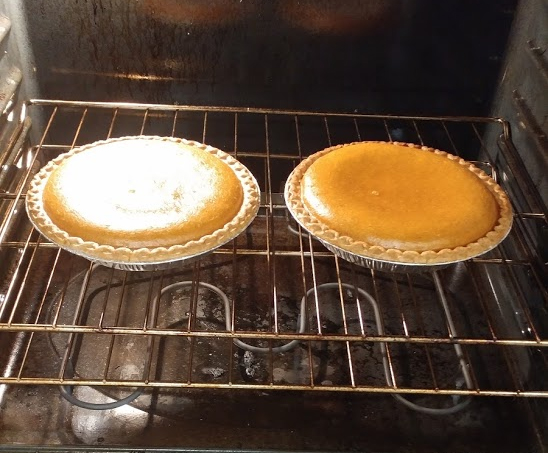
\includegraphics[height=\textheight]{pumpkin_pie/c9v9af11.jpg}}
    \end{figure}

    \introduction{
    	You can make your own crust, but my crusts aren't any better than frozen.
	}

	\ingredients[]{
		\SI{1x1/4}{cups} & Pumpkin Puree (fresh is way better but additional moisture
		adds baking time, canned is OK, but not as good) \\
		\SI{3/4}{\cup} & Sugar \\
		\SI{1/2}{\teaspoon} & Salt \\
		\SI{1/2}{\teaspoon} & Ground ginger \\
		\SI{1}{\teaspoon} & Ground cinnamon \\
		\SI{1}{\teaspoon} & All-purpose flour \\
		2 & Eggs \\
		\SI{1}{\cup} & Evaporated milk, undiluted \\
		\SI{1/2}{\teaspoon} & Vanilla extract \\
		& \SI{9}{\inch} Unbaked frozen pie crust
	}

	\preparation{
		\step In a bowl, combine the pumpkin puree, sugar, salt, ginger, cinnamon, flour and eggs. Mix until eggs are broken up.

		\step Add evaporated milk and vanilla extract, and mix until uniform.

		\step Pour into the pie crust.

		\vspace{1em}

		\step Bake at \SI{425}{\fahrenheit} (\SI{220}{\celsius}) for \SI{15}{\minute} then bake at \SI{350}{\fahrenheit} (\SI{175}{\celsius}) until the crust starts to brown
		and the pie isn't jiggly in the center when shaken (\SIrange{1x1/2}{2}{\hour},
		depending on oven and moisture).

	}

\end{recipe}